\section{Message Reachability}\label{sec:reachability}
A fundamental concept of reachability in temporal networks is the \define{time-respecting path}: a contiguous sequence of contacts with nondecreasing time. Thus, node $v$ is \define{temporally reachable} from node $u$ if there exists a time-respecting path from $u$ to $v$ \cite{Moody2002}. The following quantities are derived from the notion of a time-respecting path and help quantify reachability in a time-varying network \cite{Holme2012}.
%
\begin{itemize}
    \item The \define{influence set} $\vInfluenceSet_v$ of node $v$ is the set of nodes that $v$ can reach by a time-respecting path.
    \item The \define{source set} $\vSourceSet_v$ of node $v$ is the set of nodes that can reach $v$ by a time-respecting path.
    \item The \define{reachability ratio} $\vReachRatio(G)$ of a temporal network $G$ is the average influence-set cardinality of a node $v$.
\end{itemize}

Generally, a message-passing algorithm defines a set of constraints that determine when and what messages are sent from one node to another. Even if operating on a temporal network, those constraints may be more or less strict than requiring temporal reachability. As a dynamic process, message passing on a time-varying network requires a more general definition of reachability that can account for network topology \emph{and} message-passing semantics \cite{Barrat2013}.

Formally, the \emph{message reachability from node $u$ to node $v$} is the number of edges along the \define{shortest path} $\vPathSet$ that satisfy the message passing constraints,
%
\begin{equation*}
	\vMessageReachability(u, v) = \sum_{(i, j) \in \vPathSet} f(u, i, j, v),
\end{equation*}
%
where
%
\begin{equation*}
    f(u, i, j, v) = 
        \begin{cases}
            1 & \text{if all constraints are satisfied} \\ 
            0 & \text{otherwise.}
        \end{cases}
\end{equation*}

Node $v$ is \define{message reachable} from node $u$ if there exists a shortest path such that $\vMessageReachability(u, v) > 0$. The \define{message reachability} of node $u$ is the maximum message reachability from node $u$:
%
\begin{equation}\label{eq:vreach}
	\vMessageReachability(u) = \max_{v \in \vVertices} \, \vMessageReachability(u, v).
\end{equation}

The temporal reachability metrics previously defined can be extended to message reachability by only considering the message-reachable vertices:
%
\begin{align*}
  \vInfluenceSet_u &= \setBuilder{v \in \vVertices}{\vMessageReachability(u, v) = \card{\vPathSet}} \\
  \vSourceSet_v &= \setBuilder{u \in \vVertices}{\vMessageReachability(u, v) = \card{\vPathSet}} \\
  \vReachRatio(G) &= \sum_{v \in \vVertices} \card{\vInfluenceSet_v} \cdot \card{\vVertices}^{-1}.
\end{align*}
%
Let $\mathbf{M}$ be the \define{message reachability matrix} of the temporal network $G$ such that nodes are enumerated $1, 2, \ldots, \card{\vVertices}$ and for each $\vMessage_{ij} \in \mathbf{M}$,
%
\begin{equation*}
  \vMessage_{ij} = 
    \begin{cases}
      1 & \text{if } \vMessageReachability(i, j) = \card{\vPathSet} \\
      0 & \text{otherwise.}
    \end{cases}
\end{equation*}
%
Then the cardinality of the influence set for node $i$ is the number of nonzero elements in \indexed{i}{row of $\mathbf{M}$}:
%
\begin{equation}\label{eq:influence-size}
  \card{\vInfluenceSet_i} = \sum_{j=1}^{\card{\vVertices}} \vMessage_{ij} .
\end{equation}
%
Similarly, the cardinality of the source set for node $j$ is the number of nonzero elements in \indexed{j}{column of $\mathbf{M}$}:
%
\begin{equation}\label{eq:source-size}
  \card{\vSourceSet_j} = \sum_{i=1}^{\card{\vVertices}} \vMessage_{ij} .
\end{equation}

For risk propagation, let $\vPathSet$ is the set of edges along the shortest path from $u$ to $v$ such that the actors are enumerated $1, \ldots, \card{\vPathSet}$. Then message reachability is defined as
%
\begin{equation}\label{eq:reach}
  \vMessageReachability(u, v) = \sum_{(i, j) \in \vPathSet} [\pTransmissionRate^{i} \vScore_u > \pSendCoefficient \pTransmissionRate \vScore_{ij}] \cdot [t_u < t_{ij} + \pTimeBuffer]
\end{equation}
%
are the value and contact-time constraints in the \cShouldContactReceive[] operation (see \Cref{sec:actor-behavior}), where $(\vScore_i, t_i)$ is the current exposure score for actor $i$ and $t_{ij}$ is the most recent contact time between actors $i$ and $j$.

The value of \eqref{eq:reach} can be found by associating with each symptom score a unique identifier. If each actor maintains a log of the risk scores it receives, then the set of actors that receive the symptom score or a propagated risk score thereof can be identified. This set of actors defines the induced subgraph on which to compute \eqref{eq:reach} using a shortest-path algorithm \cite{Johnson1977}. 

Regarding efficiency, \labelcref{eq:vreach,eq:source-size,eq:influence-size} provide the means to quantify the communication overhead of a given message-passing algorithm on a temporal network. Moreover, because such metrics capture the temporality of message passing, they can better quantify complexity than traditional graph metrics.

By relaxing the constraint \eqref{eq:contact-const}, it is possible to estimate \eqref{eq:reach} with \eqref{eq:value-const}. The \define{estimated message reachability} of node $u$ to node $v$, denoted $\vEstMsgReach(u, v)$, is defined as follows. Based on \eqref{eq:value-const},
%
\begin{equation*}
  \pTransmissionRate^{\vEstMsgReach(u, v)} \cdot \vScore_u \leq \pSendCoefficient \cdot \vScore_v,
\end{equation*}
%
where the left-hand side is the value of the propagated symptom score for actor $u$ when $\vEstMsgReach(u, v) = 1$, and the right-hand side is the value required by some message-reachable actor $v$ to propagate the message received by actor $u$ or some intermediate actor. Solving for $\vEstMsgReach(u, v)$,
%
\begin{equation}\label{eq:estreach}
  \vEstMsgReach(u, v) \leq f(u, v),
\end{equation}
%
where
%
\begin{equation*}
  f(u, v) = 
  \begin{cases} 
    0 & \text{if $\vScore_u = 0$} \\
    \card{\vPathSet} & \text{if $\vScore_v = 0$} \\
    \log_{\pTransmissionRate}\pSendCoefficient + \log_{\pTransmissionRate}\vScore_v - \log_{\pTransmissionRate}\vScore_u & \text{otherwise.}
  \end{cases}
\end{equation*}
%
Equation \eqref{eq:estreach} indicates that a lower send coefficient $\pSendCoefficient$ will generally result in higher message reachability, at the cost of sending possibly ineffective messages (i.e., risk scores that do not update the exposure score of another actor). Equation \eqref{eq:estreach} also quantifies the effect of the transmission rate $\pTransmissionRate$. Unlike the send coefficient, however, the transmission rate is intended to be derived from epidemiology to quantify disease infectivity and should not be optimized to improve performance.

Given the multivariate nature of message reachability, it is helpful to visualize how it with various combinations of parameter values. \Cref{fig:reach} includes several line plots of estimated message reachability $\vEstMsgReach(u, v)$ with respect to the initial risk score magnitude of actor $u$.

\begin{figure}[htbp]
\centering
\begin{tikzpicture}
\begin{semilogyaxis}[
  xlabel={Initial risk score},
  ylabel={Send threshold},
  log ticks with fixed point,
  minor tick num=1,
  ytick={0.01, 0.05, 0.1, 0.25, 0.5, 0.75, 1},
  view={0}{90},
  colormap name=black,
  enlargelimits=0.05
]
  \addplot3 [
    contour lua={
      corners,
      levels={1,2,3,4,5,6,7,8,9,10},
      label distance=230pt,
      contour label style={
        inner sep=1pt,
        every node/.style={black, fill=white}
      }
    },
    domain=0.01:1,
    y domain=0.01:1.01,
    samples=100,
  ] {log2(y / x) / log2(0.8)};
\end{semilogyaxis}
\end{tikzpicture}
\caption[Estimated message reachability]{Estimated message reachability. Contour lines are shown for integral reachability values. Given an initial risk score and message reachability, a contour line indicates an upper bound on the permissible send threshold.}
\label{fig:reach}
\end{figure}
%
\begin{figure}[htbp]
\centering
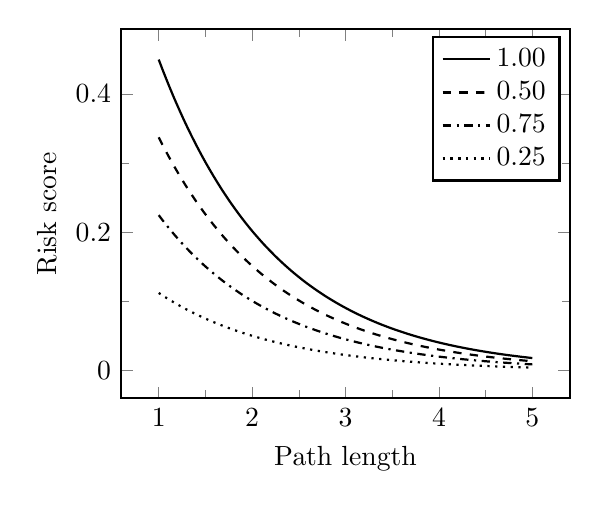
\begin{tikzpicture}
\begin{axis}[
  xlabel={Path length},
  ylabel={Risk score},
  minor tick num=1,
  width=0.6\textwidth,
  smooth,
  domain=1:5,
  y domain=0.01:1,
  samples=100,
  black,
  thick
]
  \addplot[] {e^(-0.8 * x)};
  \addplot[dashed] {0.75 * e^(-0.8 * x)};
  \addplot[dashdotted] {0.5 * e^(-0.8 * x)};
  \addplot[dotted] {0.25 * e^(-0.8 * x)};
  \legend{$1.00$, $0.50$, $0.75$, $0.25$};
\end{axis}
\end{tikzpicture}
\caption[Exponential decay of risk scores]{Exponential decay of risk scores.}
\label{fig:decay}
\end{figure}

%\section{System Model}\label{sec:system-model}

% TODO - security, privacy, mobile crowd-sensing
% TODO - centralized vs distributed - https://en.wikipedia.org/wiki/Distributed_computing
% TODO - PDAs vs local computation

%The system model is similar to that in previous work \cite{Ayday2020, Ayday2021}. \Cref{fig:actor-dataflow} illustrates the corresponding data flow\footnote{A \emph{data-flow diagram} consists of data processors (circles), directed data flow (arrows), data stores (parallel lines), and external entities (rectangles) \cite[pp. 437--438]{Fowler2004}\label{foot:dataflow}.}.
%
%\begin{itemize}
%    % TODO More conceptual detail should be introduced before this point. Add a section in the Introduction that defines self-sovereignty concepts.
%    \item Each user owns a \emph{personal data store} (PDS), a form of cloud storage that empowers the user with ownership and access control over their data.
%    \item Symptom scores are computed in a user's PDS to support integrating multiple streams of personal data \cite{Ayday2020}. While local symptom-score computation \cite{Ayday2020, Ayday2021} is more privacy-preserving, it is assumed that the user's PDS is a trusted entity.
%    \item User device interactions serve as a proxy for proximal human interactions. This work does not assume a specific protocol, but does assume that the protocol can approximate the duration of contact with relative accuracy and that communication with the actors of those contacted users can be established in a privacy-preserving manner.
%    \item No geolocation data is collected \cite{Ayday2020}. As a decentralized, proximity-based solution, it is not necessary to collect user geolocation data. See \Cref{sec:location-based} for a discussion of a geolocation-based design that was considered.
%    \item Actor-based risk propagation is a distributed, online algorithm \cite[pp. 791--818]{Cormen2022}. Previous work \cite{Ayday2020, Ayday2021} (see also \Cref{sec:previous-designs}) formulates risk propagation as a centralized, offline algorithm that periodically aggregates all user data to estimate infection risk. To improve the privacy, scalability, and responsiveness of ShareTrace, this work designs risk propagation to avoid data aggregation and to estimate infection risk in near real-time.
%\end{itemize}
%
%\begin{figure}[htb]
%    \includegraphics[width=\textwidth]{distributed-dataflow}
%    \caption[Distributed ShareTrace data flow]{Distributed ShareTrace data flow. \emph{Contacts} include the actor name and contact time of all users with which the user came into close proximity. \emph{Personal data} includes the user's demographics, reported symptoms, and diagnosis. It may also include machine-generated biomarkers and electronic health record data \cite{Ayday2020}.}
%    \label{fig:distributed-dataflow}
%\end{figure}
%
%\begin{figure}[htb]
%    \includegraphics[width=\textwidth]{centralized-dataflow}
%    \caption[Centralized ShareTrace data flow]{Centralized ShareTrace data flow. \emph{Contacts} include the actor name and contact timestamp of all users with which the user came into close proximity. \emph{Personal data} includes the user's demographics, reported symptoms, and diagnosis. It may also include machine-generated biomarkers and electronic health record data \cite{Ayday2020}.}
%    \label{fig:centralized-dataflow}
%\end{figure}